\documentclass[12pt]{report}
\usepackage{graphicx} % Required for inserting images
\linespread{1.2}

\usepackage[dvipsnames]{xcolor}
\usepackage{tikz}
\usepackage[breakable]{tcolorbox}
\appto{\bibsetup}{\raggedright}

\tikzstyle{mybox} = [draw=Dandelion, fill=Dandelion!5, ultra thick, rectangle, rounded corners, inner sep=10pt, inner ysep=15pt, text width=0.90\textwidth, align=left] 
\tikzstyle{boxtitle} = [fill=Dandelion, text=Brown, ultra thick, rectangle, rounded corners, inner sep=10pt, inner ysep=8pt, text width=0.90\textwidth]

\newcommand{\BoxDef}[2]{%
\vspace*{10px}
\noindent

\begin{center}
\begin{tikzpicture}
    \node[mybox](box){\rule{0pt}{30pt}\ignorespaces#2\unskip};
    \node[boxtitle, anchor=north west] at (box.north west) {\textbf{#1}};
\end{tikzpicture}
\end{center}
}

\usepackage[hidelinks]{hyperref}
\usepackage{amsmath}
\usepackage{amssymb}
\usepackage{bm}
\usepackage[top=2.5cm, bottom=2.5cm, left=3cm, right=3cm, centering]{geometry}
\usepackage{algorithm}
\usepackage{algpseudocode}
\usepackage{tabularx}

\begin{document}

\begin{titlepage}
\hrule
\vspace{15pt}
\begin{center}
    \Huge{\textbf{\Huge \textbf{Data Mining 2 23-24}} \\ Notes}\\
\end{center}
\vspace{15pt}
\hrule
\vfill
\hrule
\begin{center}
    \Large University of Pisa \\ M.Sc. in Data Science and Business Informatics
\end{center}
\end{titlepage}

\tableofcontents

\chapter{Rule Based Models}

A rule based classifier is a model that uses a \textbf{rule set} of ``if-then'' rules to classify instances. Each rule is expressed in the form:
\begin{equation*}
    r_i : (Cond_i) \xrightarrow{} y_i.
\end{equation*}
The left side contains a conjunction of attribute test conditions, and is called \textbf{antecedent} or \textbf{precondition}, while the right side represents the predicted class, and is called the \textbf{consequent}. Each condition is defined by a set of $k$ attribute-value pairs, such that:
\begin{equation*}
    Cond_i = (A_1 \ op \ v_1) \land (A_2 \ op \ v_2) \land \dots \land (A_k \ op \ v_k) \ ,
\end{equation*}
where $op$ is a comparison operator. Each attribute test is also known as a \textbf{conjunct}.

A rule $r$ \textbf{covers} an instance $x$ if the attributes of the instance satisfy the antecedent of the rule. Consider the following dataset:
\begin{table}[h]
    \centering
    \begin{tabular}{|c|c|c|c|}
    \hline
        Name & Can Fly & Gives Birth & Blood Type \\
    \hline
    \hline
        Bat & Y & Y & W \\
    \hline
        Owl & Y & N & W \\
    \hline
        Crocodile & N & N & C \\
    \hline
        Platypus & N & N & W \\
    \hline
    \end{tabular}
    \caption{Small example dataset.}
    \label{tab:small_dataset}
\end{table}
\\The rule $(Can Fly = Y) \land (Gives Birth = N) \xrightarrow{} Bird$ covers the instance ``Owl''.

The \textbf{coverage} of a rule is the fraction of records in the whole dataset that are covered by it. The \textbf{accuracy} (sometimes called \textbf{precision}) of a rule is the fraction of records in the dataset that satisfy the antecedent that also satisfy the consequent.
\BoxDef{Coverage and Accuracy}{
\begin{align*}
    &Coverage(r) = \dfrac{|A|}{|D|} \\\\
    &Accuracy(r) = \dfrac{|A \cap y|}{|A|}
\end{align*}
}

\section{How Rule-Based Models Work}

A rule based classifier classifies a test instance based on the rule triggered by the instance. Looking at the dataset pictured in Table \ref{tab:small_dataset}, assume we obtained the following rule set from a training set:
\begin{align*}
    &r_1 : (Can Fly = Y) \xrightarrow{} Bird \\
    &r_2 : (Gives Birth = Y) \land (Blood Type = W) \xrightarrow{} Mammal \\
    &r_3 : (Blood Type = C) \xrightarrow{} Reptile
\end{align*}
The instance Owl triggers the first rule, and is therefore classified as a $Bird$. The Bat triggers both the first and the second rule, which produce conflicting outcomes. None of the rules cover the example Platypus, so there's no immediate way to assign a class to this animal. The following section will explain how these issues can be solved.

\section{Properties of a Rule Set}

The rule set generated by the model can be characterized by the following two properties:
\BoxDef{Mutually Exclusive Rule Set}{
The rules in a rule set $R$ are mutually exclusive if no two rules in $R$ are triggered by the same instance; this property guarantees that each instance is covered by at most one rule in $R$.
}
\BoxDef{Exhaustive Rule Set}{
A rule set $R$ is exhaustive if each combination of attribute values is covered by at least one rule.
}
Unfortunately, many rule based classifiers do not have such properties. If the rule set is not exhaustive, a default rule with an empty antecedent can be added to classify all instances that are not covered by any other rule.

If the rule set is not mutually exclusive, the rules can be organized into an \textbf{ordered rule set} (also known as \textbf{decision list}).
\BoxDef{Ordered Rule Set}{
The rules in an ordered rule set $R$ are ranked in decreasing order of priority. 
}
The rank of the rule can be defined via either \textbf{rule-based ordering} (rules are ranked based on their quality, e.g., their accuracy) or \textbf{class-based ordering} (all rules that have the same consequent appear together). When a test instance is presented to the model, it is compared with the rules starting from the one at the top of the ranking, and the prediction will be the one appearing as the consequent of the highest ranking rule that covers the instance. If none of the rules are triggered, the default rule is reached, classifying the instance as the default class.

Another approach is to use a \textbf{voting scheme}, where, for each test instance, votes are accumulated for each class assigned to it by the rules it triggers. The prediction will correspond to the class with the highest number of votes, and votes may also be weighted depending on the rule that is producing it (for example, rules with lower accuracy will produce votes with lower weight).

The advantage of using an unordered rule set is that they're less susceptible to errors, since they are not biased by the chosen ordering. Model building is also less expensive, since the rules don't have to be sorted. On the other hand, classification can be more costly, since the same instance must be first compared to all the rules in the rule set before evaluating the votes.

\section{Building a Rule Set}

Rule extraction methods can be either:
\begin{itemize}
    \item \textbf{Direct}, if the rules are extracted from the data itself;
    \item \textbf{Indirect}, if the rules are extracted from some other model (e.g., Decision Trees).
\end{itemize}

\subsection{Direct Methods for Rule Extraction}

To illustrate how direct methods work, we'll consider a widely-used algorithm called \textbf{RIPPER} (Repeated Incremental Pruning to Produce Error Reduction). This algorithm scales almost linearly with the number of training examples, and is particularly suited for datasets with imbalanced class distributions. It also works well with noisy data, since it uses a validation set to prevent overfitting.

RIPPER uses the \textbf{sequential covering} algorithm to extract rules from data. This algorithm uses a greedy strategy to build rules, one class at a time. For binary problems, the majority class is chosen as the default, and the algorithm learns the rules to detect only the minority class. For multiclass problems, the classes are first ordered by prevalence in the dataset; then, starting from the least prevalent class $y_1$, all elements belonging to it are labeled as positive, while all the rest, belonging to $y_2, y_3, \dots y_c$, are labeled as negative. The sequential covering algorithm learns a set rules that discriminates between these positive and negative classes. Next, all instances in $y_2$ (the second least prevalent class) are labeled as positive, while all instances belonging to $y_3, y_4, \dots y_c$ are labeled as negative, and a new rule set is constructed. This process is repeated until only one class remains, $y_c$, which is designated as the default one.

\begin{algorithm}
\caption{Sequential covering algorithm.}
\begin{algorithmic}[1]
    \State $E$ = TR instances, $A$ = set of attribute-value pairs
    \State $Y_{\sigma} = \{y_1, y_2, \dots , y_k\}$
    \State $R = \{ \}$

    \For{each $y \in Y_{\sigma} - \{y_k\}$}
        \While{stopping cond is False}
            \State $r \xleftarrow{}$ Learn-One-Rule($E,A,y$)
            \State Remove TR instances from $E$ that are covered by $r$.
            \State $R \xleftarrow{} R \lor r$
        \EndWhile
    \EndFor
    \State Insert default rule: $R \xleftarrow{} R \lor (\{\} \xrightarrow{} y_k)$
\end{algorithmic}
\end{algorithm}

The algorithm always starts with an empty decision list, $R$, and extracts rules for each class following the ordering specified by their prevalence. The Learn-One-Rule function iteratively extracts all rules for the current class, and all training instances covered by each rule found is removed from $E$. The rule is then added to the bottom to the rule list, and the loop repeats until the specified stopping criterion is met.

\subsubsection{Rule Evaluation}

In the Learn-One-Rule function, the algorithm must search for an optimal rule by growing one in a greedy fashion. It starts with a rule with an empty antecedent, $r : \{ \} \xrightarrow{} +$. Then, new conjuncts are gradually added to the antecedent in order to improve the rule's accuracy.

RIPPER uses the \textbf{FOIL's First Order Inductive Learner) information gain} as the measure to choose which conjunctive to add to the rule's antecedent.

\BoxDef{FOIL's Information Gain}{
Given $p_0$ and $n_0$ the number of positive and negative examples covered by the original rule, and $p_1$ and $n_1$ the number of positive and negative examples covered by the new rule, the FOIL's information gain is defined as:
\begin{equation*}
    FOIL's \ inf. gain = p_1 \times \left( \log_2 \dfrac{p_1}{p_1 + n_1} - \log_2 \dfrac{p_0}{p_0 + n_0} \right)
\end{equation*}
}
RIPPER starts with a rule $r : A \xrightarrow{} +$. It then adds one conjunct, $B$, generating the rule $r : A \land B \xrightarrow{} +$, and the information gain is calculated for this addition. This step is repeated for different conjuncts, and the rule with the highest information gain is chosen to replace the original rule. The function stops once there's no additions that improve the information gain, so the rule covers only positive instances. Additionally, all instances covered by the rule are removed from the training set.

RIPPER also performs pruning of the rules to improve the generalization error based on their performance on a validation set. After generating a rule, the following metric is computed:
\begin{equation*}
    v = \dfrac{(p-n)}{(p+n)} \ ,
\end{equation*}
where $p$/$n$ are the number of positive/negative validation instances covered by that rule. If this measure improves after removing a conjunct, the latter is permanently pruned, and the measure is again evaluated for the next conjunct. The check follows the reverse order to the one established by the insertion of conjuncts during generation. Note that a pruned rule may cover both positive and negative examples of the training set; this means that the rule is less adapted to the training data, but performs better on unseen examples. 

The generation of rules is interrupted once a stopping condition is verified, such that the complexity of the model is high enough to generalize well, but not so high that it overfits the training data. Some common stopping conditions are evaluated based on the \textbf{Minimum Description Length} (\textbf{MDL}). The MDL measures the cost of a model as:
\begin{equation*}
    Cost(M, D) = Cost(D|M) + \alpha \times Cost(M) \ ,
\end{equation*}
where $M$ and $D$ are the model and the data, respectively, and $\alpha$ is a tuning hyperparameter (usually set to 0.5).  The first term of the addition encodes the misclassification error, while the second term uses node encoding (number of children) plus encoding of the splitting condition. The cost is evaluated in terms of how many bits are needed to encode the rule set: if the addition of a rule would increase the length of the set by at least $d$ bits, then RIPPER stops adding rules (by default, $d$ is 64 bits). This is a form of Pessimistic Error Estimate, since it evaluates the generalization error of the model as:
\begin{equation*}
    R(T) = R_{emp} + \Omega \times \dfrac{k}{l} \ ,
\end{equation*}
where $R_{emp}(T)$ is the training error, $\Omega$ is a trade-off hyperparameter that represents the cost of adding a new rule, $k$ is the size of the rule set, and $l$ is the number of training instances.

RIPPER also performs additional optimization steps to determine whether the rules in the set can be replaced by better alternatives. For each rule $r$, two new rules are considered as replacement:
\begin{itemize}
    \item A replacement rule $r^*$: a new rule is grown from scratch;
    \item A revised rule $r'$: conjuncts are added to the rule $r$ to extend it.
\end{itemize}
The rule set for $r$ is compared with the rule sets for $r^*$ and $r'$, choosing the rule that minimizes the MDL.

\subsection{Indirect Methods for Rule Extraction}

Indirect methods generate a rule set by using the output of some other model, typically an unpruned decision tree. In a decision tree, each path connecting the root to a leaf can be expressed as a classification rule, where each attribute test condition encountered on the path is a different conjunct of the antecedent, and the (majority) class in the leaf node is the consequent. This section will focus on the approach followed by the algorithm C4.5rules.

A rule is generated from each path in the tree. For each rule $r : A \xrightarrow{} y$ in the rule set, alternative rules $r' : A' \xleftarrow{} y$ are considered, where $A'$ is obtained by removing one of the conjuncts in $A$. The simplified rule with the lowest pessimistic error rate is retained as a replacement if the error rate is also lower than that of the original rule. Eventual duplicates of the new rule are eliminated from the rule set.

After generating the rule set, C4.5rules uses a class-based ordering to rearrange the rules, so that all rules predicting the same class appear close together in the same subset. The description length of each subset is calculated, and the classes are arranged in increasing order of their total description length. This way, the subset with the lowest description length is given priority over the others, since it is assumed to contain the best set of rules.

\section{Characteristics of Rule Based Models}

Rule based classifiers are very similar to decision trees, and have about the same expressiveness. Both models construct rectilinear decision boundaries in the input space, and assign a class to each partition. Rule based classifiers, however, can allow multiple rules to be triggered for the same instance, while in decision trees, each instance can only follow one specific path. Because of this, rule based models can approximate more complex functions.

Like decision trees, they can handle different types of attributes, both continuous and categorical, and can work for both binary and multiclass classification tasks. Additionally, rule based classifiers often produce models that are easier to interpret but have comparable performance to decision trees.

They can also handle redundant attributes, since if two or more highly correlated, only one of them is chosen to be added as a conjunct. Since irrelevant attributes will show poor information gain, rule based models will tend to avoid choosing them as conjuncts. Still, as seen for decision trees, if the problem is sufficiently complex, sometimes irrelevant attributes may be chosen over other more relevant ones that show poor information gain individually, but would be useful when interacting with others.

They cannot handle missing values in the test set, as the positioning of the rules in a rule set follows a specific ordering strategy, so if a test instance is covered by multiple rules they may produce conflicting outputs.

Since RIPPER uses a class-based ordering strategy, emphasizing classes with fewer instances, these models are very well suited for imbalanced class distributions. 
\chapter{Sequential Pattern Mining}

Sequential pattern mining is the discovery of subsequences that frequently appear in a sequential dataset, i.e., finding all the subsequences whose number of occurrences is greater or equal than a user-defined threshold ($minsup$). These frequent subsequences are also called \textbf{sequential patterns}. Unlike frequent itemset mining, sequences also contain spatio-temporal information that specifies when certain transactions happen. Common examples of sequential data may be the purchase history of customers in a supermarket, genome sequences, or web browsing history. 

\BoxDef{Sequence, element, event}{
    A sequence $s$ is an \textbf{ordered} list of elements $s = \langle e_1 e_2 \ldots e_n\rangle$. Each element (or ``transaction'') $e_j$ is an \textbf{ordered} list of one or more events (or ``items'') $e_j = \{ i_1, i_2, \ldots , i_m \}$. Each event is a literal.
}
Each event/item can occur only once in an element/transaction, but may occur multiple times in separate elements/transactions. Events in the same element appear according to lexicographical ordering. An example of a sequence is the following:
\begin{equation*}
    s = \langle \{1, 2, 3\} \{1\} \{1, 3\} \rangle \,.
\end{equation*}
The whole sequence is delimited by angle brackets $<,>$, and each element is delimited by curly brackets $\{,\}$.
This sequence contains three elements, three unique events, and a total of 6 events.
The \textbf{length} of a sequence ($|s|$) is the number of its elements. The \textbf{size} of the sequence is the total number of its events. A sequence of size $k$ is also known as a \textbf{$k$-sequence}.

\BoxDef{Subsequence}{
    A sequence $s = \langle s_1 s_2 \ldots s_n\rangle$ is a subsequence of a sequence $t = \langle t_1 t_2 \dots t_m\rangle$ if there exist integers $1 \leq i_1 < i_2 < \dots < i_k \leq n $ such that $s_1 \subseteq t_{i_1}, s_2 \subseteq t_{i_2}, \dots , s_n \subseteq t_{i_k}$.
}
If $s$ is a subsequence of $t$, then $s$ is \textbf{contained} in $t$.

Let \textit{D} be a dataset of one or more sequences, called data-sequences. Each data-sequence consists in a list of elements, ordered by increasing time. Each element is associated with a sequence-id, a timestamp, and a list of the events it contains. For simplicity, we will assume that elements occur at regular intervals and never overlap. For each pattern, we can calculate its \textbf{support} and \textbf{support count}, defined the same as they were defined for itemsets in association analysis.

\BoxDef{Support}{
    The support of a sequence $s$ is the fraction of data-sequences in a dataset $D$ that contain $s$.
}
\BoxDef{Support Count}{
    The support count of a sequence $s$ is the absolute number of data-sequences in a dataset $D$ that contain $s$.
}

For the purpose of sequential pattern mining, only a single valid occurrence of a sequence in a data-sequence is considered towards computing support, so even if a subsequence appears in $n$ different ways within the same data-sequence, its support count will only be increased by 1. We can now formally define sequential pattern mining as follows:
\BoxDef{Sequential Pattern Mining}{
    Given \textit{D} a dataset of data-sequences, and $minsup$ a user-defined minimum support threshold, the problem of mining sequential patterns
    is to find all sequences whose support $\geq minsup$; each such sequence is a \textbf{sequential pattern}, also called frequent sequence. 
}

Discovering all frequent sequences in a dataset is a computationally challenging task. The most basic algorithm that solves the problem uses a brute-force approach: generate all possible $k$-sequences for $k = 1,2,3 \ldots$, and compute support for every single one of them. The ones whose support is greater or equal than a $minsup$ threshold are declared frequent. However, the set of all possible candidate sequences is exponentially large and difficult to enumerate, even more than what was seen in association analysis. An event can appear multiple times in different elements within the same sequence, and elements arranged in different orders correspond to different sequences. This means that even when considering a relatively small set of events, the algorithm generates a large set of candidates; e.g., with only three unique events, the candidates generated for size $k = 2$ would be:
\begin{gather*}
    \langle\{i_1\} \{i_1\}\rangle, \langle\{i_1\} \{i_2\}\rangle, \langle\{i_1\} \{i_3\}\rangle, \langle\{i_1 i_2\}\rangle, \langle\{i_1 i_3\}\rangle \\ 
    \langle\{i_2\} \{i_1\}\rangle, \langle\{i_2\} \{i_2\}\rangle, \langle\{i_2\} \{i_3\}\rangle, \langle\{i_2 i_3\}\rangle \\
    \langle\{i_3\} \{i_1\}\rangle, \langle\{i_3\} \{i_2\}\rangle, \langle\{i_3\} \{i_3\}\rangle \,,
\end{gather*}
for a total of 12 candidates. As the number of items increases (it can easily be in the order of the hundreds, thousands, or more), the number of candidates would explode beyond what could be analyzed in appropriate time. Even if we were to generate candidates from input sequences, removing one item at a time and calculating support, we would still have a disproportionate amount of sequences to check.

One approach to solve the problem efficiently is to exploit the anti-monotonicity property of support and the Apriori property, already used for frequent itemset mining. As a reminder:
\BoxDef{Anti-monotone property}{
A measure $f$ possesses the anti-monotone property if for every itemset $X$ that is a proper subset of an itemset $Y$, it holds that $f(Y) \leq f(X)$.
}

\BoxDef{Apriori principle}{
    If a $k$-sequence is frequent, then all of its $k-1$-subsequences must also be frequent.
}

\section{Time Constraints}
\label{sec:tconstr}

Time constraints control how support is calculated by considering the time elapsed between elements of a sequence. For example, consider a dataset that represents market basket data: each product is an event, each individual purchase is an element, and each data-sequence is a set of purchases made by a customer within some interval of time (months or years). If we're interested in finding a correlation between certain products, we may want to limit the time passed between transactions: if a customer bought product $A$, and then bought product $B$ several months after, then the sequence $\langle \{A\} \{B\} \rangle$ is not significant for the purposes of our analysis. The time constraints are three: \textbf{maxspan}, \textbf{maxgap}, and \textbf{mingap}.

\BoxDef{maxspan}{
The $maxspan$ constraint specifies the maximum time passed between the first and last element of a sequence. If $t_{i,i+1}$ is the time passed between consecutive elements $i$ and $i+1$ of a data-sequence, then the following inequality must hold true:

\begin{equation*}
	\sum t_{i,i+1} \leq maxspan
\end{equation*}
}

\BoxDef{maxgap and mingap}{
The $maxgap$ and $mingap$ constraints specify the maximum time and minimum time passed between two consecutive elements of a sequence, respectively. If $t_{i,i+1}$ is the time passed between consecutive elements $i$ and $i+1$ of a data-sequence of length $n$, then the following inequality must hold true for $i = 1 \ldots (n-1)$:

\begin{equation*}
    mingap < t_{i,i+1} \leq maxgap
\end{equation*}
}
The $maxgap$ constraint violates the Apriori principle. A modification of this principle is used instead, which refers to \textbf{contiguous subsequences}: 

\BoxDef{Contiguous Subsequence}{
Given a sequence $s = \langle s_1s_2 \ldots s_n \rangle$, a sequence $t$ is a contiguous subsequence of $s$ if:

	\begin{itemize}
		\item $t$ is obtained by dropping an event from either $s_1$ or $s_n$;
		\item $t$ is obtained by dropping one event from any element $s_i$ that contains more than one event;
		\item $t$ is a contiguous subsequence of $w$, and $w$ is a contiguous subsequence of $s$.
	\end{itemize}
}
The Apriori principle can then be modified in the following way:
\BoxDef{Modified Apriori Principle}{
If a $k$-sequence is frequent, then all of its \textbf{contiguous} $k-1$-subsequences must also be frequent.
}

\section{Generalized Sequential Patterns Algorithm}

the Generalized Sequential Patterns (GSP) algorithm is an efficient algorithm that uses the anti-monotonicity of support to extract sequential patterns; it also supports time constraints. It is very similar to the Apriori algorithm, with the same exact basic structure. The pseudocode of the algorithm is presented in the next pseudocode block.

\begin{algorithm}
\caption{Generalized Sequential Patterns pseudocode.}
\begin{algorithmic}[1]
    \State $k=1$.
    \State $F_k = \{ i : i \in I \land s(i) >= minsup \}$ \# find all frequent 1-sequences
    \Repeat
        \State $k = k + 1$
        \State $C_k$ = \texttt{candidate-gen}
        \State $C_k$ = \texttt{candidate-prune}($C_k$, $F_{k-1}$)

        \For{all $t \in T$}
            \State $C_t$ = \texttt{subsequences}($C_k$, $t$)

            \For{all $c \in C_t$}
                \State $\sigma(c) = \sigma(c) + 1$
            \EndFor
        \EndFor

        \State $F_k = \{ c | c \in C_k \land s(c) \geq minsup \}$ \# find all frequent k-sequences
    \Until{$F_k = \emptyset$}
\end{algorithmic}
\end{algorithm}
The algorithm does a first pass over the dataset and computes support for all unique events, determining which 1-sequences (sequences with only a 1-event element) are frequent. The main loop of the algorithm has a candidate generation phase, a candidate pruning phase, and finally a support counting phase.

\subsection{Candidate generation}

This phase generates new candidate $k$-sequences by merging together the frequent $(k-1)$-sequences found in the previous iteration. There's two possible cases: 
\begin{itemize}
    \item For $k = 2$, all frequent 1-sequences are merged with each other (including with themselves). For each couple of events $i_1$ and $i_2$, the generated candidates will be: $\langle\{i_1\} \{i_2\}\rangle$, $\langle\{i_2\} \{i_1\}\rangle$, and $\langle\{i_1 i_2\}\rangle$, if $i_1 \neq i_2$; only $\langle\{i_1\} \{i_2\}\rangle$, if $i_1 = i_2$.

    \item For $k > 2$, two frequent $(k-1)$-sequences $s_1$ and $s_2$ are merged only if the subsequence obtained by dropping the first event from $s_1$ is the same as the one obtained by dropping the last event from $s_2$. Then, the candidate can be generated in two ways. 
    
    If the last element of $s_2$ has only one event, append that last element to $s_1$ and obtain the merged sequence.
    
    If the last element of $s_2$ has more than one event, append the last event of that last element to the last element of $s_1$ and obtain the merged sequence.
\end{itemize}
Note that a sequence can, in some cases, be merged with itself, as long as the conditions described above hold true. Also, this procedure is both complete and generates no duplicates.

\subsection{Candidate Pruning}

A $k$-candidate can be pruned if at least one of its $(k-1)$-subsequences is infrequent, since support shows anti-monotone property, and therefore its support can only be less-or-equal-than any of its subsequences. Pruning is done by dropping one event at a time from the $k$-candidate, and checking if the resulting $(k-1)$-sequence is contained in the frequent ones found in the previous iteration. If any of them are not frequent, the candidate can be discarded.

\subsection{Support Counting}

After the candidate set is pruned, the algorithm iterates over the data-sequences, and for each of them finds which $k$-candidates it contains, increasing their support count accordingly. At the end, all $k$-candidates whose support is less than $minsup$ are discarded, while the rest form the set of frequent $k$-sequences.

\section{Generalized Sequential Patterns and Time Constraints}

Introducing the $mingap$, $maxgap$, and $maxspan$ time constraints requires the support counting and candidate pruning procedures to be modified. Support counting must now consider the time gap between consecutive elements (for the $mingap$ and $maxgap$ constraints) and the overall span of the sequence (for the $maxspan$ constraint) when determining if a candidate is contained in a sequence. This means that the procedure can't simply determine the first occurrence of a candidate within a data-sequence, but must keep searching for an occurrence that satisfies all three constraints at once, such that $mingap < t_{i,i+1} \leq maxgap$, and $\sum t_{i,i+1} \leq maxspan$, where $t_{i,i+1}$ is the gap between consecutive elements in a data-sequence.

As for candidate pruning, the Apriori principle and anti-monotonicity of support no longer hold true because of the $maxgap$ constraint. If a candidate $c$ is being pruned, and all of its subsequences are checked, some of them may be infrequent, even though the candidate is actually a frequent sequence.

For example, let sequence $s = \langle \{1, 2\} \{2\} \{3\} \{4\} \rangle$ be a data-sequence, and sequence $c = \langle \{1\} \{2\} \{4\} \rangle$ a candidate sequence. If $maxgap = 2$, then $c$ is contained in $s$, but the subsequence $c' = \langle \{1\} \{4\} \rangle$ is not, because the gap between $\{1\}$ and $\{4\}$ is $3$.

Therefore, the procedure must check all of a candidate's contiguous subsequences, removing one event at a time only from the elements that contain two events or more. If at least one of the contiguous subsequences of a candidate is infrequent, the candidate can be pruned. This new pruning strategy ensures that no candidate frequent sequences are accidentally discarded, since it skips all the elements that, when removed, could produce a sequence that contains a gap between consecutive elements that violates the $maxgap$ constraint. However, this strategy inevitably decreases the effect that pruning has on the overall execution.
\chapter{Transactional Clustering}

Clustering is a task whose objective is to find grouping of objects of a dataset into sets, called clusters, where each member of a cluster is more similar to all other elements in the same cluster than it is to elements in different clusters. For numerical data, proximity between objects is measured using distances, typically Euclidean or Manhattan, since records with numerical attributes only can be interpreted as points in an $n$ dimensional space. However, these measures are not appropriate to carry clustering tasks on categorical attributes, which are used to represent transactional data. The biggest issue is that the way two transactions are deemed ``near'' each other does not correspond to geometrical proximity.

This issue can be illustrated with a simple example. Assume we have 4 transactions:
\begin{align*}
    &T1 = \{1,2,3,4\} \\
    &T2 = \{1,2,4\} \\
    &T3 = \{3\} \\
    &T4 = \{4\}
\end{align*}
Usually, transactional data can be represented with a set of boolean attributes, one for each item, where a value of ``1'' indicates the presence of the corresponding item, while a ``0'' indicates its' absence. In this case, the dataset will be represented as:
\begin{align*}
    &P1 = \{1,1,1,1\} \\
    &P2 = \{1,1,0,1\} \\
    &P3 = \{0,0,1,0\} \\
    &P4 = \{0,0,0,1\} \\
\end{align*}
If Euclidean distance were used to calculate how far or close there transactions are to each other, we would find out that the distance between transactions 3 and 4 is:
\begin{equation*}
    d(P3, P4) = \sqrt{(0)^2 + (0)^2 + (1)^2 + (-1)^2} = \sqrt{2}    
\end{equation*}
However, the two transactions don't share any item, making them completely different.

This chapter will present four different algorithms that can cluster categorical data, each of which define proximity between transactions in different ways.

\section{K-Modes}

K-modes is similar to K-means, but can be used for categorical attributes. It starts by randomly choosing $k$ data points at random to elect to representative points. The algorithm then enters a loop, in which it assigns all points to the closest mode, recomputes the mode of each cluster, and repeats the past two steps until no object changes assignment between two successive iterations (or until some stopping criterion is verified).

The distance between two records is calculated as the number of mismatches between their attributes:
\begin{gather*}
    d(X,Y) = \sum_i \delta(x_i, y_i) \\
    \delta(x,y) = \begin{cases}
        0 & (x = y) \\
        1 & else
    \end{cases}
\end{gather*}
The representative object of a cluster is calculated as the mode of the objects in the same cluster.

This algorithm minimizes the function:
\begin{equation*}
    P(W,Q) = \sum_{i}^k \sum_{j}^n w_{i,j} d(x_i, Q_i) \,,
\end{equation*}
where $w_{i,j}$ is 1 if object $i$ belongs to cluster $j$, 0 otherwise, and $Q$ is the set of the modes of each cluster.

\section{ROCK (RObust Clustering using linK)}

ROCK is a hierarchical algorithm that uses \textbf{neighborhoods} and \textbf{links to clusters} to define closeness between two transactions. Neighborhoods are calculated locally, while links are calculated globally. The algorithm can be split into three main parts:
\begin{enumerate}
    \item \textbf{A random sample is drawn from the dataset}. A sample of points is uniformly extracted, using it to form clusters instead of the entire data. This ensures the algorithm can be used even on very large dataset while still producing an accurate enough clustering.

    \item \textbf{An agglomerative hierarchical clustering algorithm is performed on the sample}. ROCK follows the same steps as other hierarchical agglomerative algorithms: it starts by assigning each point to a singleton cluster, then computes the similarity measure for all pairs of clusters, and merges the two ``closest'' objects. These steps repeat until some stopping condition is met (usually, until $k$ clusters are formed).

    Two objects $A$ and $B$ are \textbf{neighbors} if their similarity is greater or equal than some hyperparameter threshold $\theta$, chosen between 0 and 1:
    \begin{equation*}
        A \in N_B \land B \in N_A \iff sim(A,B) \geq \theta \,,
    \end{equation*}
    where similarity is calculated with Jaccard's coefficient (the ratio of the number of matching items between the objects and the total number of distinct items between the two):
    \begin{equation*}
        sim(A,B) = \dfrac{|A \cap B|}{|A \cup B|}
    \end{equation*}
    A point is also considered a neighbor of itself.

    A \textbf{link} is calculated as the number of common neighbors between two objects:
    \begin{equation*}
        link(A,B) = |N_A \cap N_B|
    \end{equation*}
    Higher values of link means that there's a higher probability that the two objects belong to the same group (since they share neighbors). 
    
    \item \textbf{The entire dataset is labeled by assigning each object to a cluster}. A random sample is selected from each cluster, and each point $p$ in the original dataset is assigned to the cluster $i$ such that $p$ has the maximum number of neighbors in the corresponding sample.
\end{enumerate}
The best clusters are the ones that maximize the criterion function of the algorithm:
\begin{align*}
    &E_l = \sum_{i=1}^k n_i \sum_{p_q,p_r \in C_i} \dfrac{link(p_q, p_r)}{n_i^{1 + 2 f(\theta)}} \,, \\
    & f(\theta) = \dfrac{1-\theta}{1+\theta}
\end{align*}
where $n_i$ is the size of cluster $C_i$. This function penalizes clusters that present very few links compared to the expected number of links in the entire cluster, so that we avoid that objects with a low number of links are assigned to the same cluster. At each merging step of the algorithm, the two clusters that are merged are the ones that maximize the goodness measure:
\begin{equation*}
    g(C_i, C_j) = \dfrac{link(C_i, C_j)}{(n_i + n_j)^{1+2f(\theta)} - n_i^{1+2f(\theta)} - n_j^{1+2f(\theta)}} \,,
\end{equation*}
where the numerator is the number of cross-links between the two clusters, and the denominator is the expected number of them.

\section{CLOPE (Clustering with sLOPE)}

CLOPE is a clustering algorithm that is efficient for high dimensional data. It uses an exclusively global criterion function that tries to increase the intra-cluster overlap of transactions. This is done by increasing the height-to-width ratio of the cluster histogram. It is especially suitable for big datasets with a high number of unique items, since it uses an array representation of the data instead of binary.

For each cluster, the width is calculated as the number of distinct items, while the height is calculated as the ratio between the total number of (non unique) items and the width. In the example below, the cluster has a width of 5 and a height of 2.4.
\begin{figure}[h]
    \centering
    \begin{minipage}{0.49\textwidth}
    \centering
    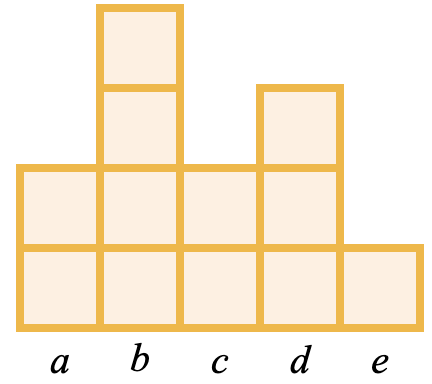
\includegraphics[width=0.5\linewidth]{img/CLOPE_cluster.png}
    \begin{equation*}
        C_i = \{abcd, bcd, ab, bde\}
    \end{equation*}
    \end{minipage}
\hfill
    \begin{minipage}{0.49\textwidth}
        \begin{gather*}
            W(C_i) = 5 \\
            S(C_i) = 12 \\
            H(C_i) = \dfrac{12}{5} = 2.4
        \end{gather*}
    \end{minipage}
\end{figure} \\
Higher ratios of height/width mean higher item overlapping.

The goodness of a clustering is calculated as the \textbf{gradient} of each cluster:
\begin{equation*}
    Profit_r(C) = \dfrac{\sum_{i=1}^k \dfrac{S(C_i)}{W(C_i)^r} \times |C_i|}{\sum_{i=1}^k |C_i|}
\end{equation*}
The hyperparameter $r$ is called \textbf{repulsion}; for higher values of $r$, transactions within the same cluster must share a large portion of items, while for lower values transactions may share a lower amount of items, which can be useful for sparse databases.

The algorithm has two phases: first, each transaction is added to a new cluster or to an existing one such that the profit is maximized. Then, for each transaction, it is checked whether moving it to a different cluster improves profit, repeating this step until all transactions remain in the same cluster (no moves will improve the profit).

\section{TX-Means}

TX-Means is a parameter-free transactional clustering algorithm, and is useful to partition data obtained from a massive amount of different datasets. It finds a representative transaction for each cluster, which summarizes the pattern presented by the elements of that cluster. Like X-Means, it starts out with a cluster that contains all the objects in the dataset, and chooses how to recursively split it into subpartitions by using the Bayesian Information Criterion.
\begin{algorithm}
\caption{TX-Means pseudocode.}
\begin{algorithmic}[1]
    \State $r$ = \texttt{getRepr}($B$) \# get representative basket of entire set of baskets
    \State $r$ is added to queue $Q$

    \While{$Q \neq \emptyset$}
        \State $C, r$ are extracted from $Q$
        \State Common items are removed from $C$ and $r$
        \State $C1,C2,r1,r2$ = \texttt{bisectBasket}($C$)
        \If{$BIC(C1,C2,r1,r2) > BIC(C,r)$}
            \State Add $C1,C2,r1,r2$ to $Q$
        \Else
            \State Add $C, r$ to result 
        \EndIf
    \EndWhile

    \State Return result
\end{algorithmic}
\end{algorithm} \\
The algorithm starts by finding a representative for all objects in the dataset, then enters a loop in which each cluster currently in the queue is split. Each split is either accepted, reinserting the new subpartitions in the queue, or rejected, adding the parent cluster to the result, depending on whether it produces an improvement in the BIC score. Below is the pseudocode for the functions \texttt{getRepr()} and \texttt{bisectBasket()}.

\begin{algorithm}[H]
\caption{\texttt{getRepr} pseudocode.}
\begin{algorithmic}[1]
    \State $I$ = set of items not shared among all baskets in $B$
    \State $r$ = set of items in common to all baskets in $B$
    \State Calculate frequencies of items in $I$
    \State $i = 0$, $d_0 = \inf$
    \While{$I \neq \emptyset$}
        \State $i = i + 1$
        \State Add the items in $I$ with maximum frequency to $r$
        \State Calculate the distance $d_i$ between $r$ and the baskets in $B$ via Jaccard coefficient
        \If{$d_i \geq d_{i-1}$}
            \State Return $r$
        \Else
            \State Remove from $I$ items with maximum frequency
        \EndIf
    \EndWhile 
    \State Return $r$
\end{algorithmic}

\end{algorithm}
\begin{algorithm}
\caption{\texttt{bisectBasket} pseudocode.}
\begin{algorithmic}[1]
    \State $SSE = \inf$
    \State Select two random baskets $r1,r2$
    \While{True}
        \State $C1,C2$ = clusters obtained by assigning baskets to either $r1$ or $r2$
        \State $r1_{new}$ = \texttt{getRepr}($C1$)
        \State $r2_{new}$ = \texttt{getRepr}($C2$)
        \State $SSE_{new} = SSE(C1,C2,r1_{new},r2_{new})$
        \If{$SSE_{new} \geq SSE$}
            \State Return $C1,C2,r1,r2$
        \EndIf
        \State $r1 = r1_{new}$
        \State $r2 = r2_{new}$
    \EndWhile
\end{algorithmic}
\end{algorithm}
TX-Means is also scalable thanks to the following sampling strategy. A random subset of transactions is chosen from the dataset, and TX-Means is run on that subset, returning a set of clusters and their respective representative transactions. Then, all the remaining transactions in the dataset are assigned to the clusters using a nearest neighbor approach with respect to the representatives found by the algorithm.

\nocite{*}
\bibliographystyle{unsrt}
\clearpage\bibliography{bibliography}

\end{document}
